\documentclass{beamer}
\usepackage[utf8]{inputenc}
\usetheme{Madrid}
\usecolortheme{default}
\usepackage{amsmath,amssymb,amsfonts,amsthm}
\usepackage{txfonts}
\usepackage{tkz-euclide}
\usepackage{listings}
\usepackage{adjustbox}
\usepackage{array}
\usepackage{tabularx}
\usepackage{gvv}
\usepackage{lmodern}
\usepackage{circuitikz}
\usepackage{tikz}
\usepackage{graphicx}

\setbeamertemplate{page number in head/foot}[totalframenumber]

\usepackage{tcolorbox}
\tcbuselibrary{minted,breakable,xparse,skins}



\definecolor{bg}{gray}{0.95}
\DeclareTCBListing{mintedbox}{O{}m!O{}}{%
  breakable=true,
  listing engine=minted,
  listing only,
  minted language=#2,
  minted style=default,
  minted options={%
    linenos,
    gobble=0,
    breaklines=true,
    breakafter=,,
    fontsize=\small,
    numbersep=8pt,
    #1},
  boxsep=0pt,
  left skip=0pt,
  right skip=0pt,
  left=25pt,
  right=0pt,
  top=3pt,
  bottom=3pt,
  arc=5pt,
  leftrule=0pt,
  rightrule=0pt,
  bottomrule=2pt,
  toprule=2pt,
  colback=bg,
  colframe=orange!70,
  enhanced,
  overlay={%
    \begin{tcbclipinterior}
    \fill[orange!20!white] (frame.south west) rectangle ([xshift=20pt]frame.north west);
    \end{tcbclipinterior}},
  #3,
}
\lstset{
    language=C,
    basicstyle=\ttfamily\small,
    keywordstyle=\color{blue},
    stringstyle=\color{orange},
    commentstyle=\color{green!60!black},
    numbers=left,
    numberstyle=\tiny\color{gray},
    breaklines=true,
    showstringspaces=false,
}
%------------------------------------------------------------
%This block of code defines the information to appear in the
%Title page
\title %optional
{2.2.26}

%\subtitle{A short story}

\author % (optional)
{BALU-ai25btech11017}



\begin{document}


\frame{\titlepage}
\begin{frame}{Question}
Find the area of the triangle formed by the points $P(-1.5,3)$, $Q(6,-2)$ and $R(-3,4)$.
\\ 
\end{frame}



\begin{frame}{Theoretical Solution}

Given three points\\
\begin{align}
  \vec{P}=\begin{myvec}{-1.5\\3}\end{myvec}\;
  \vec{Q}=\begin{myvec}{6\\-2}\end{myvec}\;
  \vec{R}=\begin{myvec}{-3\\4}\end{myvec}\
   \end{align}
   \begin{align}
 \vec{Q}-\vec{P}=\begin{myvec}{7.5\\-5}\end{myvec}\
\end{align}
\begin{align}
  \vec{R}-\vec{P}=\begin{myvec}{-1.5\\1}\end{myvec}\
\end{align}
\begin{align}
ar(PQR) &= \frac{1}{2} \, \|(\vec{Q} - \vec{P}) \times (\vec{R} - \vec{P}) \|
\end{align}
\begin{align}
ar(PQR) &= \frac{1}{2} \, \|(\vec{Q} - \vec{P}) \times (\vec{R} - \vec{P}) \|=0
\end{align}
points are collinear
\end{frame}
\begin{frame}[fragile]
    \frametitle{C Code}

    \begin{lstlisting}
#include <stdio.h>
#include <math.h>

// Function to calculate area of triangle using cross product
double triangle_area(double P[2], double Q[2], double R[2]) {
    double x1 = Q[0] - P[0];
    double y1 = Q[1] - P[1];
    double x2 = R[0] - P[0];
    double y2 = R[1] - P[1];
    
    // Cross product magnitude in 2D
    double cross = fabs(x1 * y2 - y1 * x2);
    
    return 0.5 * cross;
}



   

     \end{lstlisting}
\end{frame}
\begin{frame}[fragile]
    \frametitle{C Code - Resultant velocity}

    \begin{lstlisting}
  int main() {
    double P[2] = {-1.5, 3};
    double Q[2] = {6, -2};
    double R[2] = {-3, 4};

    double area = triangle_area(P, Q, R);
    
    printf("Area of triangle PQR = %.2f\n", area);
    
    return 0;
}

    \end{lstlisting}
\end{frame}
\begin{frame}[fragile]
    \frametitle{Python Code}
    \begin{lstlisting}
import matplotlib.pyplot as plt   # ✅ Import first

# Coordinates of the points
P = (-1.5, 3)
Q = (6, -2)
R = (-3, 4)

# Function to calculate area of triangle
def triangle_area(p, q, r):
    x1, y1 = p
    x2, y2 = q
    x3, y3 = r
    return 0.5 * abs(x1*(y2-y3) + x2*(y3-y1) + x3*(y1-y2))

# Calculate area
area = triangle_area(P, Q, R)
print(f"Area of triangle PQR = {area}")









    \end{lstlisting}
\end{frame}

\begin{frame}[fragile]
    \frametitle{Python Code}
    \begin{lstlisting}
# Plotting
plt.figure(figsize=(6,6))
x_vals = [P[0], Q[0], R[0], P[0]]
y_vals = [P[1], Q[1], R[1], P[1]]

plt.plot(x_vals, y_vals, 'b-o', label=f"Triangle PQR (Area = {area})")
plt.scatter([P[0], Q[0], R[0]], [P[1], Q[1], R[1]], color='red')

# Annotate points
plt.text(P[0]+0.2, P[1], f"P{P}")
plt.text(Q[0]+0.2, Q[1], f"Q{Q}")
plt.text(R[0]+0.2, R[1], f"R{R}")

    \end{lstlisting}
\end{frame}

\begin{frame}[fragile]
    \frametitle{Python Code}
    \begin{lstlisting}
plt.title("Triangle formed by P, Q, R")
plt.axhline(0, color='black', linewidth=0.5)
plt.axvline(0, color='black', linewidth=0.5)
plt.grid(True)
plt.legend()
plt.axis("equal")

# Save as picture
plt.savefig("triangle_pqr.png")   # Saves in current folder
plt.show()

    \end{lstlisting}
\end{frame}

\begin{frame}{Plot}
    \centering
    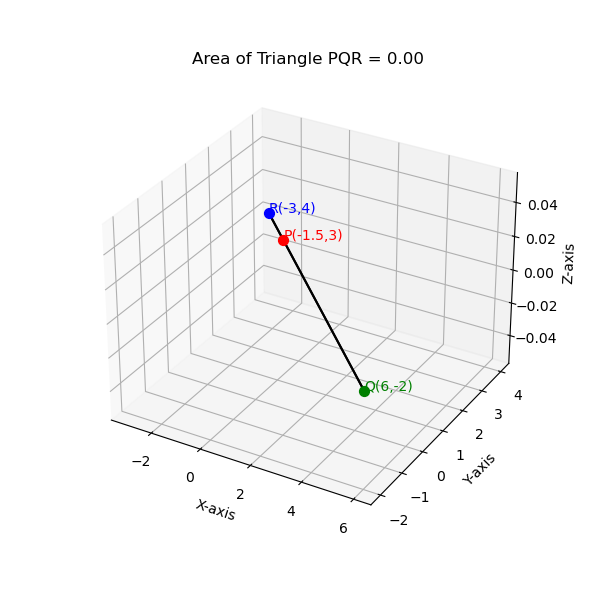
\includegraphics[width=\columnwidth, height=0.8\textheight, keepaspectratio]{figs/fig4.png}     
\end{frame}




\end{document}